\chapter{特定の時空間への進入時に自動センシングするアプリケーション}
\thispagestyle{myheadings}
本章では特定の時空間への進入時に自動センシングするアプリケーションについて述べる.
\ref{lavlusReq}章ではまずラヴラスのモバイルアプリケーションの要求仕様を定義する.
\ref{myApp}章では特定の時空間への進入時に自動センシングするアプリケーションの実装に述べる.
\ref{myApp_STF}章では時空間フェンシングの実装について述べる.
\ref{myApp_notify}章ではセンシング依頼通知の実装について述べる.
\ref{myApp_sensing}章では自動センシングの実装について述べる.


\section{ラヴラスのモバイルアプリケーションの要求仕様}
\label{lavlusReq}
ラヴラスのモバイルアプリはセンシングプロジェクトダウンロード,時空間フェンシング,センシング依頼の承諾,自動的にセンシング,Wi-Fi環境下で自動的にアップロードができる必要がある.
協力者の物理的コストを軽減させるために,協力者への通知と協力者自身の操作の低減や,端末のデータ通信量を圧迫しない必要がある.
センシングプロジェクトをダウンロードする時,端末の通信量とデータ容量を圧迫しない為に,協力者が参加する可能性があるセンシングプロジェクトのみダウンロードする必要がある.
また,センシングが終わった後,Wi-Fiに接続している時に自動でアップロードされる必要がある.
協力者の物理的コストを軽減させるために,協力者へ通知と協力者自身の操作を最小限に抑える必要がある.
依頼者の制作したセンシングプロジェクトに参加する可能性が高い協力者のみにセンシング依頼通知を送る必要がある.
例えば,時空間に近いもしくはすでに進入している場合である.
また,一度センシング依頼に承諾,拒否した場合そのセンシングプロジェクトから通知は発行されない.
時空間に進入している間,バックグラウンドで自動でセンシングされる必要がある.
協力者の心理的コストを軽減するために,協力者はすでに承諾したセンシングプロジェクトへの拒否や,既にアップロードしたセンサデータに削除申請が出せる必要がある.
本アプリはクラウドセンシングプラットフォームとして,多くのセンサに対応する必要がある.
また,アップロードされるセンサデータは協力者のプライバシを侵害しない為に,匿名化及び抽象化する必要がある.

% 協力者が本アプリを起動,もしくは起動してから一定時間毎にサーバからセンシングプロジェクトをダウンロードする.
% あいまいな位置情報
% 協力者が時空間に進入した場合,通知が発行され,センシング依頼画面が立ち上がる.センシング依頼に承諾した場合,時空間に進入している間,バックグラウンドで自動でセンシングされる.
% センシングが終わった後,Wi-Fiに接続している時に自動でアップロードされる.
% 協力者はすでにセンシングに承諾したセンシングプロジェクトにもセンシング拒否ができる.
% また,送信したセンサデータに削除申請ができる.



\section{特定の時空間への進入時に自動センシングするアプリケーションの実装}
\label{myApp}
依頼者の制作したセンシングプロジェクトに対応したセンシングをするためにモバイルアプリを実装する.
作成するモバイルアプリの候補としてiOSとAndroidアプリがある.
本研究で作成するアプリはクラウドセンシングプラットフォームとして多くのセンサに対応する必要がある.
そのため,iOSと比べて多くのセンサを取り扱えるAndroidアプリを作成した.
本アプリは4.1章で述べた内,時空間フェンシング,センシング依頼の承諾,自動的にセンシングのみ実装した.

\begin{figure}[tbh]
    \centering
    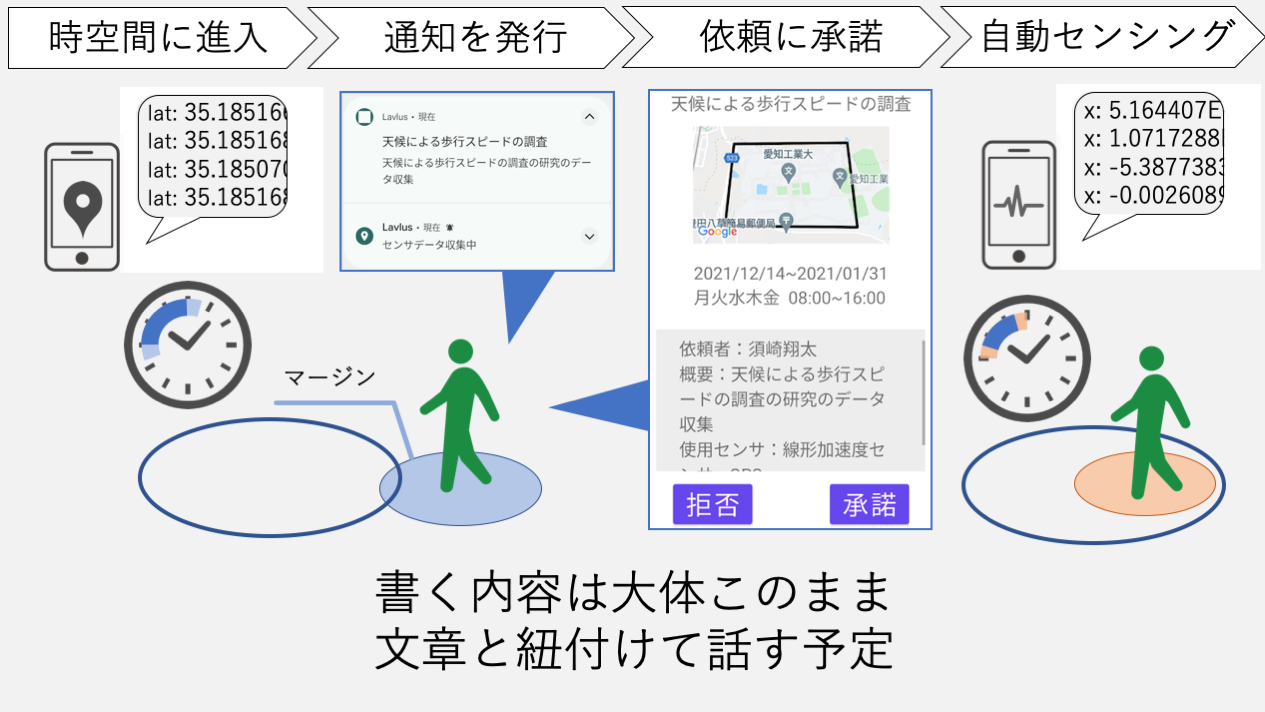
\includegraphics[width=16cm]{img_myApp.png}
    \caption{特定の時空間への進入時に自動センシングするアプリケーションの全体図}
    \label{fig:myApp}
\end{figure}

実装したアプリの全体図を図\ref{fig:myApp}に示す.

\subsection{時空間フェンシングの実装}
\label{myApp_STF}
ジオフェンシングには緯度経度,BLEビーコン,Wi-Fiなどが使われる.
ラヴラスではジオフェンシングを確実に認識する必要がある.
そのため,今回は依頼者と協力者が視覚的に認識しやすい緯度経度を採用した.
% 時空間に進入しているかの判定のため,一定間毎に位置情報を現在時刻を取得する.

ジオフェンスが緯線,経線に並行な線のみでできている長方形の場合,条件分岐を用いてジオフェンシングが可能である.
現在位置の緯度がジオフェンスの最北端よりも低く最南端よりも高い,また経度が指定エリアの最東端よりも低く最西端よりも高い場合,ジオフェンス内にいると判定する.
この条件分岐を用いると,正常にジオフェンシングできるのは緯度経度と平行な辺のみで構成されている矩形のみとなる.
ラヴラスのユースケースとして,特定の施設や建物などを対象とする場合があり,多くの施設や建物は緯度経度に並行ではない.
緯度経度に並行ではない場合,条件分岐では正確なジオフェンシングができない.
例えば,ジオフェンスがひし形の場合を想定する.

\begin{figure}[tbh]
    \centering
    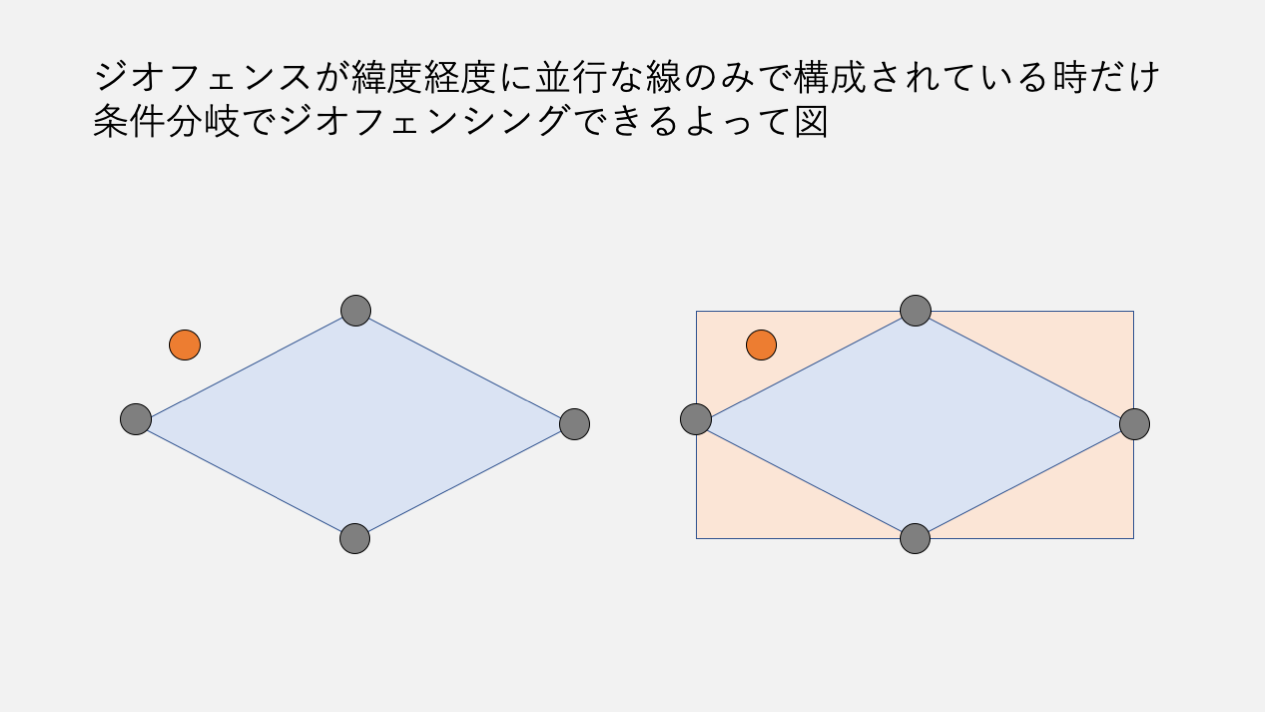
\includegraphics[width=16cm]{img_polygon_1.png}
    \caption{条件分岐を用いたジオフェンシング}
    \label{fig:polygon_1}
\end{figure}

\begin{figure}[tbh]
    \centering
    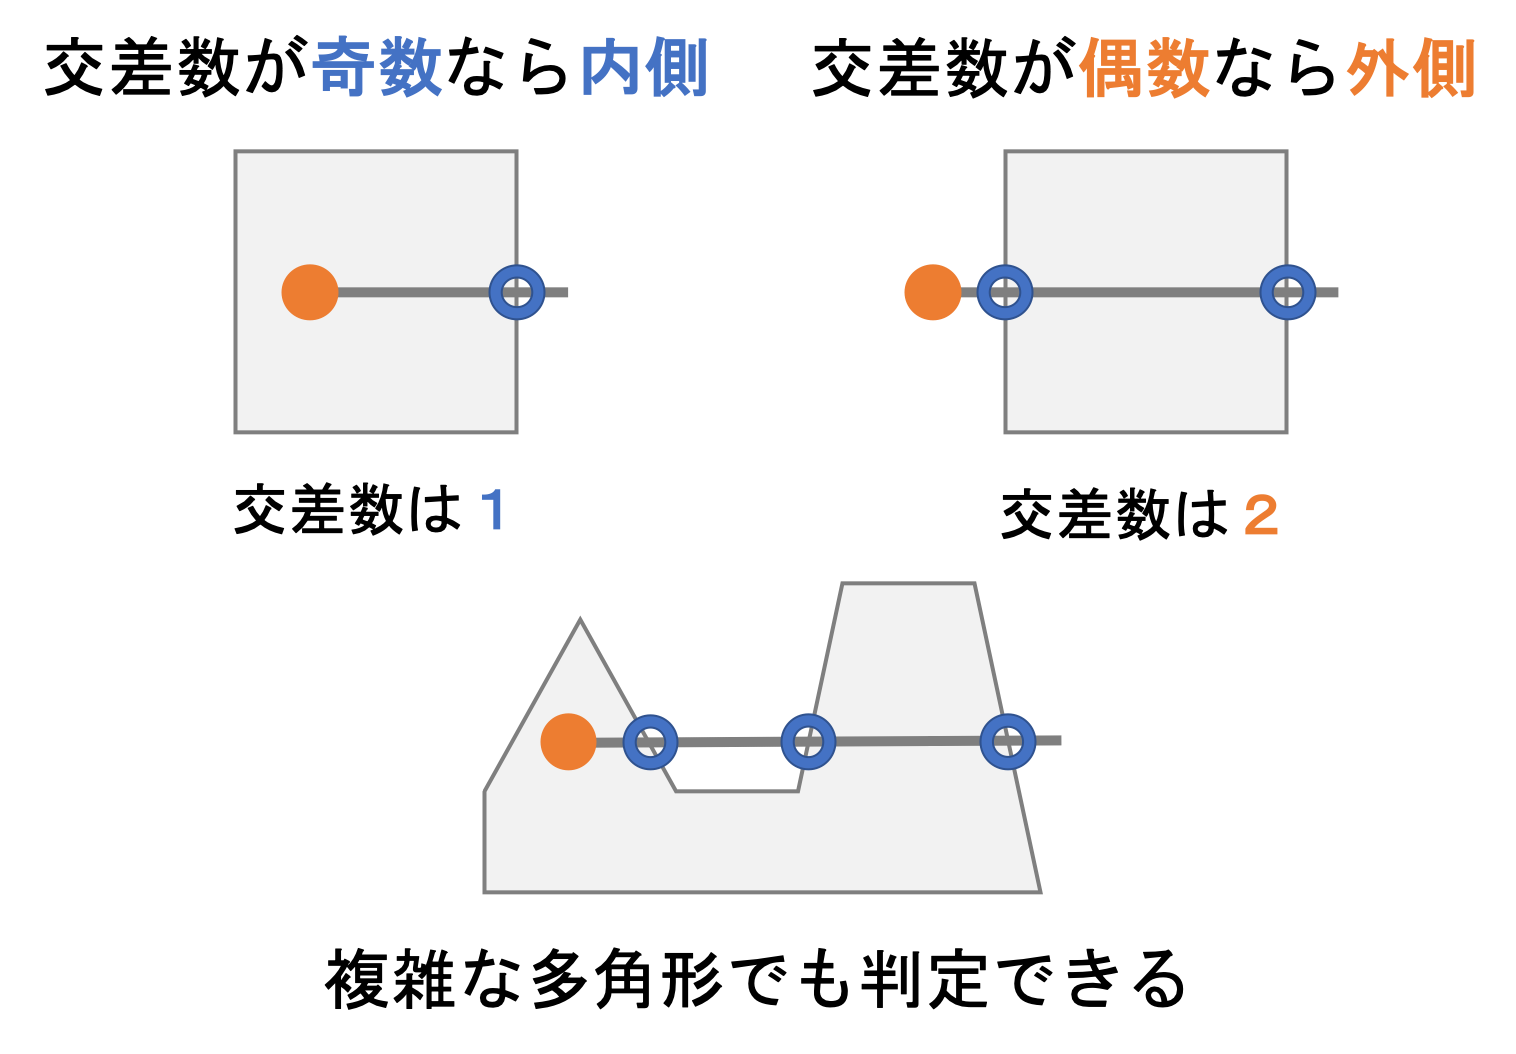
\includegraphics[width=16cm]{img_polygon_2.png}
    \caption{点の内外判定を用いたジオフェンシング}
    \label{fig:polygon_2}
\end{figure}

正常なエリア判定としては,図\ref{fig:polygon_1}左の通り現在地(赤丸)にいた場合はエリア内に進入していないため,通知は送られないはずである.
しかし,条件分岐を用いたエリア判定の場合は,ひし形の外側にひし形の頂点を辺の中心とした矩形の判定エリアが形成されるため,図\ref{fig:polygon_1}右のように現在地がエリア内にいると判定され,誤って通知が送られてしまう.
このように,条件分岐を用いると自ずとジオフェンスが矩形になってしまう.

ジオフェンスが複雑な矩形な場合に対応するためにポリゴンの内外判定アルゴリズム\cite{naigai}を使用する.
点の多角形に対する内外判定を図\ref{fig:polygon_2}に示す.
点の内外判定とは,まず点(青丸)から多角形に対して線を引く.
この時引く線は直線であれば,どの方向に引いても良い.
その線と多角形との交点(赤丸)の数が奇数個であれば多角形よりも内側にいる,偶数個であれば多角形よりも外側にいると判定できる.
この場合,丁度線と多角形の辺が重なったり,線と多角形の頂点と重なると,誤った判定を行ってしまう.
しかし,緯度経度は小数点以下が7桁もあり,位置情報は変化し続けるため,丁度重なる場合は今回考えないものとしている.
依頼者が図\ref{fig:polygon_2}のようにどれだけ複雑な多角形のエリアを設定しても,内部か否かは判定可能である.
今回は実装は行っていないが円のようなエリアでも判定は可能である.
また,今回はGPSのみを用いたエリア判定のため,平面的なエリア判定しか行えない.
1階や2階などの立体的なエリア判定は今後の課題とする.

確実に時空間に進入した場合のみセンシングする,時空間に進入する可能性が高い協力者にセンシング依頼通知を発行するなど,様々なシチュエーションに対応するため,時空間の拡大と縮小が可能なマージンを実装した.

\begin{figure}[tbh]
    \centering
    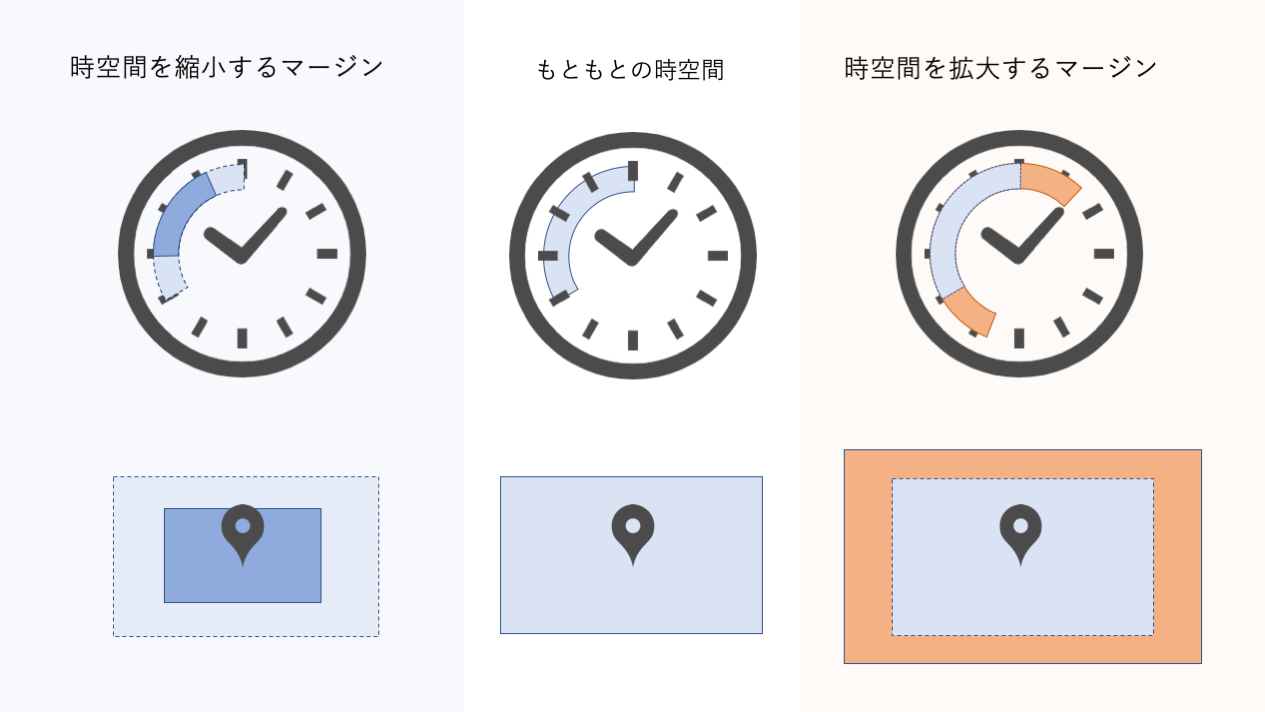
\includegraphics[width=16cm]{img_margin_1.png}
    \caption{時空間を拡大縮小するマージンの例}
    \label{fig:margin_1}
\end{figure}

時空間を拡大縮小するマージンの例を図\ref{fig:margin_1}に示す.
ジオフェンスが緯線,経線に並行な線のみでできている長方形の場合,加算と減算を用いてマージンの実装が可能である.
ジオフェンスを拡大する場合は,最北端の緯度と最東端の経度に加算し最南端の緯度と最西端の経度に減算する.
ジオフェンスを縮小する場合は,最北端の緯度と最東端の経度に減算し最南端の緯度と最西端の経度に加算する.
しかし,本アプリはジオフェンスが複雑な矩形に対応する必要がある.
ジオフェンスが複雑な矩形の場合に対応するため,ジオフェンスではなく協力者にマージンを持たせた.

\begin{figure}[tbh]
    \centering
    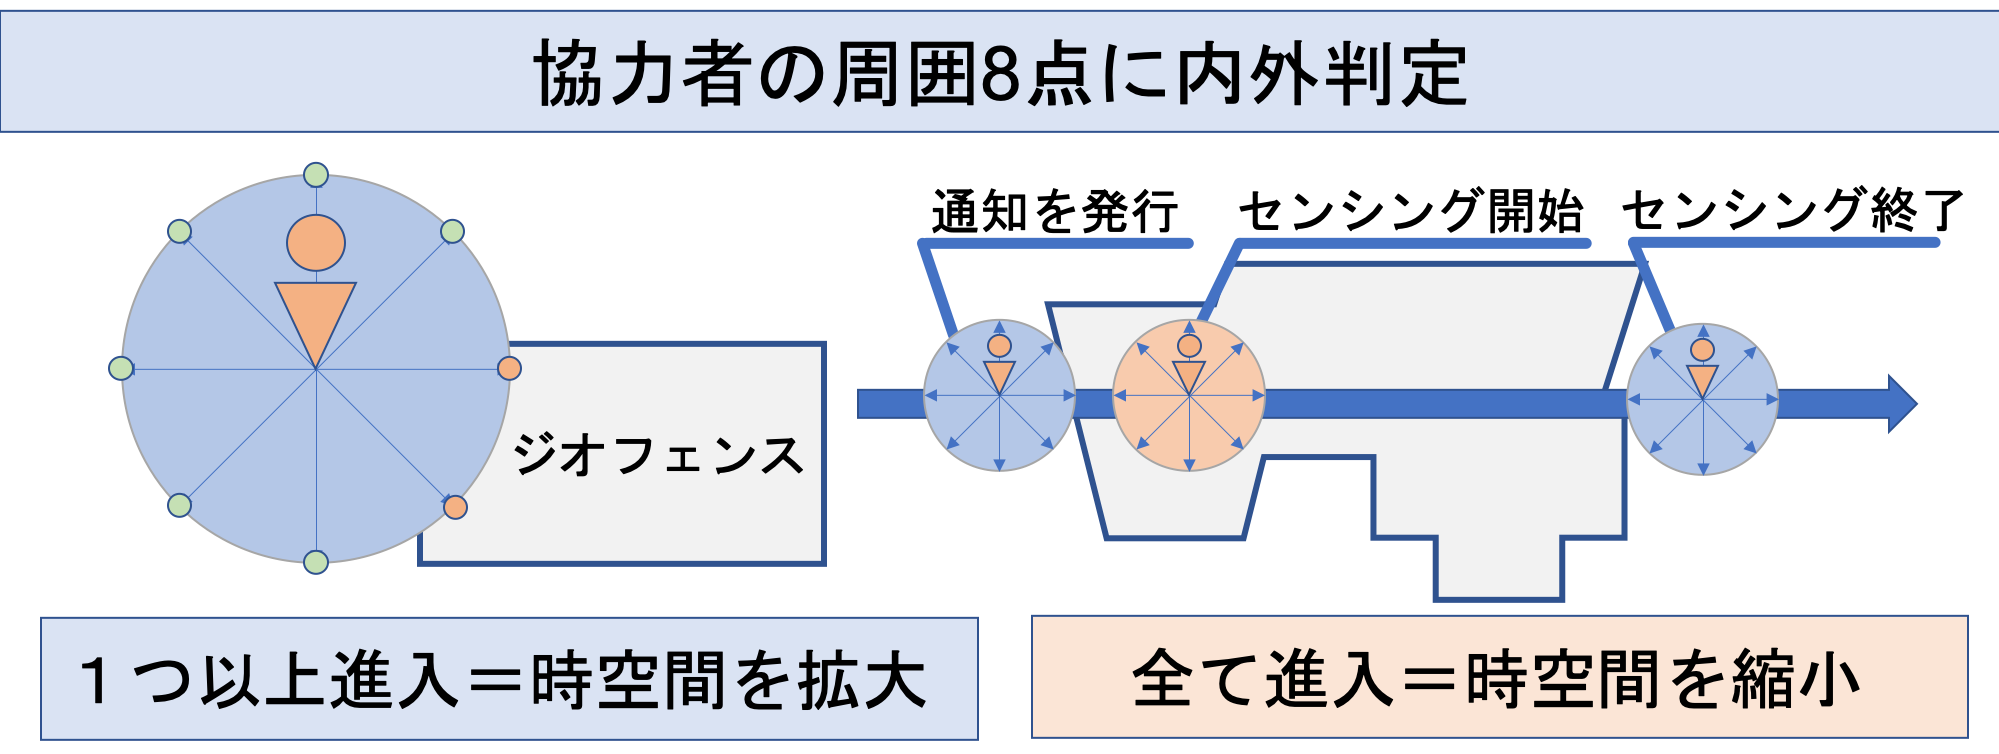
\includegraphics[width=16cm]{img_margin_2.png}
    \caption{時空間を拡大縮小するマージン}
    \label{fig:margin_2}
\end{figure}

協力者に対するマージンを図\ref{fig:margin_2}に示す.
協力者の現在位置から上下左右斜めに8つの点を作る.
ジオフェンスを拡大する場合は,8つの点のうち1つでもジオフェンシングに進入している時に進入していると判定する.
ジオフェンスを縮小する場合は,8つの点が全てジオフェンシングに進入している時に進入していると判定する.
これにより,どれだけ複雑な矩形でもマージンを持たせられる.

% ジオフェンスに緯度経度を使用しているため,ジオフェンスのマージンの距離を緯度経度に変換する必要がある.


% 緯度経度の距離の話,複雑な矩形の話,


% 複雑な矩形のマージンに対応できるように端末にマージンを設けた.

\subsection{センシング依頼通知の実装}
\label{myApp_notify}
協力者へのセンシング依頼通知を減らすために,センシング依頼通知はクラウドセンシングに参加する可能性が高い協力者に発行する.
センシングプロジェクトに設定された時空間に近い協力者を,そのクラウドセンシングに参加する可能性が高いとする.
例えば,すでに始まっているクラウドセンシングの付近にいる協力者や,もうすぐ自分がいる場所でクラウドセンシングが始まる協力者である.
なので,時空間を広げるようにマージンを取り,その時空間へ進入した場合,通知を発行する.
センシングプロジェクトに設定された空間から離れた場所にいる協力者はそのクラウドセンシングに参加する可能性が低いとする.
例えば,すでに始まっているクラウドセンシングから離れた場所にいる協力者である.
クラウドセンシングに参加する可能性が低い協力者に通知を発行しても,クラウドセンシングに参加する可能性が低く,たとえセンシング依頼に承諾しても,センサデータがもらえる可能性が低い.
また,協力者は参加しないクラウドセンシングの通知が何度も発行されると不快に感じる可能性がある.
すでにジオフェンスに進入していても,数日後や数ヶ月後など大きく時間が離れている場合も通知を発行しない.
旅行や出張などで遠出している協力者が旅行先で,数ヶ月後に行われるクラウドセンシングの通知を受け取っても参加する可能性が低い.
自宅や職場の付近で,数ヶ月後に行われるクラウドセンシングは,協力者が参加する可能性が低くない.
しかし,普段から設定されたジオフェンスに近づく場合,そもそもクラウドセンシングに参加する可能性が高いため,数日前,数ヶ月前に通知を発行する必要はない.
また,センシング依頼に承諾してから数日すると,協力者は承諾したクラウドセンシングについて忘れる可能性がある.

\begin{figure}[tbh]
    \centering
    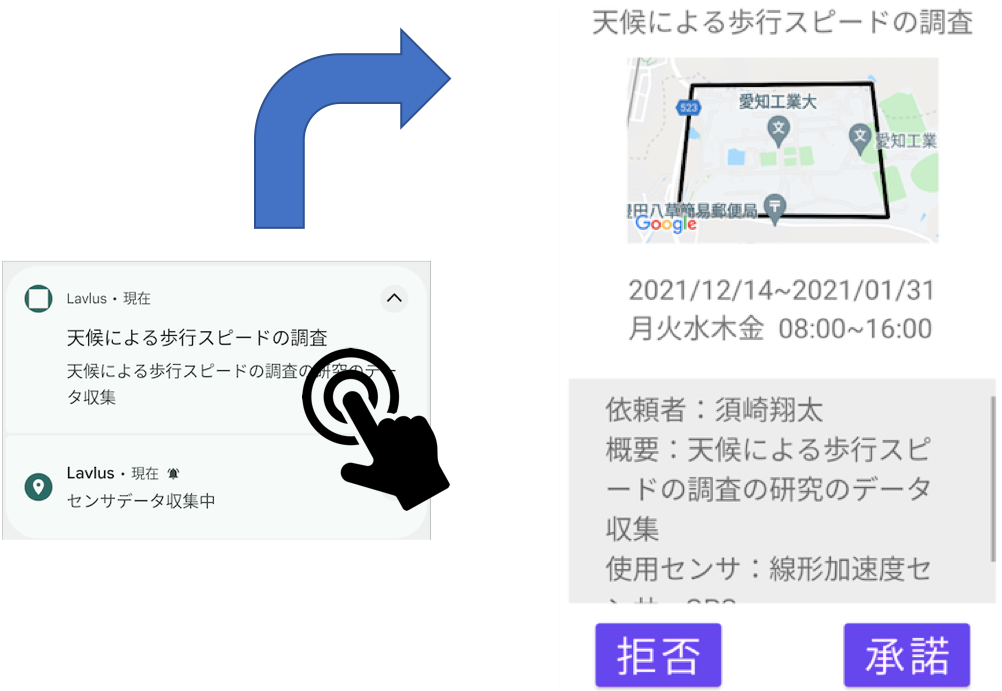
\includegraphics[width=16cm]{img_notify.png}
    \caption{発行される通知とセンシング依頼画面の例}
    \label{fig:notify}
\end{figure}


協力者がセンシング依頼通知をタップすると,センシング依頼画面が立ち上がり,依頼者の名前や使用するセンサ,時空間が提示される(図\ref{fig:notify}).
協力者に対するジオフェンスの提示はAndroidアプリと親和性の高いGoogleMapを使用している.
協力者がセンシング依頼通知を開いた時,ジオフェンスを瞬時に認識するために,GoogleMapにジオフェンスの境界線を引き,GoogleMapのズームレベルを調整している.
GoogleMapはジオフェンスの中央を中心に表示されている.
ジオフェンスの中央の緯度は最北端と最南端,経度は最東端と最西端の平均から求めている.
GoogleMapはジオフェンスを全て表示するズームレベルに設定される.
最北端と最南端から縦の長さ,最東端と最西端から横の長さを計算し,ズームレベル毎のピクセルと距離の関係\cite{GoogleMap}を参考に適切なズームレベルを算出する.

協力者が提示された情報に納得し協力すると判断した場合,協力者はセンシング承諾ボタンを押してクラウドセンシングに協力する.
協力者はセンシング依頼画面に提示される情報を確認する.
この時,協力者は提示された情報に少しでも不信感を覚えたり,納得できない場合はセンシング拒否ボタンを押してクラウドセンシングに協力しない.



\subsection{自動センシングの実装}
\label{myApp_sensing}
% 入った時と出た時でマージンが違う.
% どう言った時でセンシングが始まるべきか,おわるべきか.
協力者の操作を低減させる為,協力者が時空間に進入し,センシング依頼に承諾している場合,バックグラウンドで自動にセンシングされる.
そのため,協力者はスマホアプリを意識して開く必要はなく,アプリケーション自体を終了させなければ,途中でセンシングは終了しない.
バックグラウンドにより,協力者の操作などの負担の軽減に加え,センシングをしているという感覚を意識させないため,より普段の振る舞いをセンシングできる.

確実に協力者の時空間への進入,退出を判定するため,進入時は時空間を狭くするマージン,退出時は時空間を広くするマージンを取る.
ジオフェンシングの境界付近かつ,位置情報が不安定になると進入,退出の判定を繰り返してしまう.
これを防ぐためにマージンを取る.
しかし,時空間が小さい場合,狭くするマージンを取りすぎると時空間に進入しづらく,または進入できなくなってしまう.
例えば縦横どちらかが10m以下のジオフェンスに対して狭くするマージンを5m以上取ると進入できなくなる.
同様に時間を狭くするマージンを設定された時間より多くとってしまうと進入できなくなる.
そのため時空間を狭くするときのマージンは時空間の大きさを考慮する必要がある.
現時点でマージンはセンシングプロジェクト毎に設定している.

クラウドセンシングプラットフォームとして多くのセンサと自由な周波数に対応し,プライバシを侵害するセンサデータは抽象化した.
さまざまなクラウドセンシングに対応するために多くのセンサと周波数に対応する必要がある.
例えば,歩行推定では加速度センサ,気圧センサ,角速度センサ,位置情報などが必要になる可能性がある.
騒音計測では音センサ,環境測定では温度や湿度が必要になる可能性がある.
センサの種類だけではなく,自由に設定できる周波数も必要である.
同じセンサでも,用途によって周波数はさまざまである.
例えば,気圧センサを歩行推定に使う場合,高い周波数でセンシングする.
一方,天候推定では高い周波数でセンシングする必要がないため,低い周波数でセンシングする.
依頼者が作成するセンシングプロジェクトにはセンサの種類とセンサ毎の周波数が設定されている.
本アプリではセンシングプロジェクトに沿って,複数のセンサとセンサ周波数に対応したセンシングができる.
例えば,加速度を50Hz,気圧を10Hzでセンシングなど,周波数をセンサ単位で設定できる.
また,同時に複数の時空間に進入して,複数のクラウドセンシングに参加する場合がある.
本アプリはセンシングプロジェクト毎にセンサの種類とその周波数を管理しているため,同時に複数のセンシングが可能である.
例えば,加速度を50Hzで取るクラウドセンシグと20Hzでとるクラウドセンシングに協力した場合でも適当にセンシングできる.


% その為,プライバシを侵害する可能性が高いセンサデータは抽象化されている.
% ジオフェンシングの境界付近かつ,位置情報が不安定になると進入,退出の判定を繰り返してしまう.


% Local Variables: 
% mode: japanese-LaTeX
% TeX-master: "root"
% End: 
